\documentclass[14pt,a4paper]{article}
\usepackage[utf8]{inputenc}
\usepackage[T1]{fontenc}
\usepackage{amsmath}
\usepackage{amsfonts}
\usepackage{amssymb}
\usepackage{graphicx}
\usepackage{hyperref}
\usepackage[style=authoryear,backend=biber]{biblatex}
\DeclareDelimFormat{postnotedelim}{\addcomma\space}
\usepackage{csquotes}
\usepackage[margin=3.5cm]{geometry}
\usepackage{titlesec}
\usepackage{appendix}
\usepackage{booktabs}
\usepackage{longtable}
\usepackage{fancyhdr}
\usepackage{pdfpages}
\usepackage{xurl}

\addbibresource{references.bib}

\titleformat{\section}
  {\normalfont\Large\bfseries}{\thesection}{1em}{}
\titleformat{\subsection}
  {\normalfont\large\bfseries}{\thesubsection}{1em}{}

\title{Testing Strategy and Evidence}
\author{for Verification and Validation of Group 4's Operational BPMN Model}
\date{}

\renewcommand{\labelitemi}{-}

\pagestyle{fancy}
\fancyhf{}
\renewcommand{\headrulewidth}{0.4pt}
\renewcommand{\footrulewidth}{0.4pt}
\fancyhead[L]{UFCFAF-30-3 | Development of Information Systems Projects}
\fancyhead[R]{Page \thepage}
\fancyfoot[C]{\thepage}

\begin{document}

\maketitle

\hrule

\vspace{3em}

Word Count: 1166

\vspace{3em}
\hrule

\vspace{2em}
\textbf{Abstract}
\vspace{1em}

A comprehensive testing strategy for the Car Repair Shop, focussing on the verification and validation of BPMN process automations. Through a systematic and rigorous test methodology we ensure both technical correctness and successfully converge for all hard goals and key business objectives.

Please be aware there is an Appendix A attached to the end of this document with a complete and fully implemented test suite log.

\vspace{3em}
\hrule

\thispagestyle{empty}

\tableofcontents
\pagenumbering{roman}

\newpage

\pagenumbering{arabic}

\section{Introduction}

Testing process-driven applications presents unique challenges compared to traditional software validation. As \textit{\parencite[p. 127]{Bozkurt2013}} observe, "process implementations span organisational boundaries and combine human tasks with automated services," creating distinct and demanding verification requirements.

This paper outlines the systematic testing strategy for Group 4's Car Repair Shop, verifying the integrity of the operational BPMN model. The approach employs what \textit{\parencite[p. 219]{Giray2016}} describe as "multi-dimensional verification techniques" that address technical consistency, ensuring that automated processes work, look, and feel the way they are intended for as many, if not all, of possible outcomes as can be achieved.


\section{Testing Strategy Framework}

\subsection{Test Derivation from Requirements}

The testing strategy employed a goal-based test derivation methodology, extracting test cases directly from operational BPMN processes. Following \textit{\parencite[p. 176]{Kunze2015}}' approach, each test is aligned with specific goals and quality attributes to ensure that "verification activities directly validate stakeholder intentions rather than merely technical correctness."

\subsection{Layered Testing Architecture}

For the most part, and to test as exhaustively as we needed to, we stuck to a three-layer test plan.

\begin{enumerate}
    \item \textbf{Unit Testing}
    \item \textbf{Integration Testing}
    \item \textbf{System Testing}
\end{enumerate}

This layered approach follows \textit{\parencite[p. 92]{Garcia-Borgonon2017}}' recommendation for process applications, ensuring "progressive verification from technical correctness to business alignment." Each layer employs specific testing techniques appropriate to its scope and objectives, as detailed in subsequent sections. As well as this, it is important to keep in mind input validation for forms and what we refer to as `Layer Zero' in this scenario (by which we mean a preemptive safeguard to a lot of type errors, and runtime failures easily avoided with some Regular Expressions).

\section{Unit, Integration, System Testing}

Unit testing involves validating desirable outcomes on an individual process tasks, gateways, and even the state of some variables basis to verify correct behaviour in isolation. In reality, individual ad hoc unit tests were carried out on specific variables, gateways, and operational paths all throughout development and also in the final integration testing of all features in all manner of states, however we did not implement any rigorous regimen or set schema with respect to JUnit5 as we had originally planned. Despite this seemingly inefficient choice, time was invested in coding features, and once features were implemented they were seldom changed because they worked so well. The addition of formal unit tests did not appeal given the scope of the project. In our case we ran the risk of breaking the code in order to implement the tests and so we procrastinated on doing so. This was in some respects our greatest failure, however our monolith works well!

To add insult to this injury, the final product would have been easily transferable to a structure suiting JUnit testing, however given that the automation met all business needs and provided working output, fully satisfying the case study, and that there were no considerations for future maintainability or sustainability - neither new features nor code changes to be added, we felt that unit testing became almost unnecessary for our needs. Too small a safeguard on a project not large enough to warrant them.

To put it into perspective, we utilised Anthropic's Claude 3.7 Large Language Model with extended thinking capability to vet and implement a large number of features with many manual alterations after the fact, but condensing our 2000 line mini-monolith Zeebe Worker down into smaller modular chunks was always and still is (just about) on the verge of being but one prompt away from a set of testable, modular units. Around 2000 lines of code at the current state of the art is, for certain as of April 1st 2025, the absolute limit of Claude's output capability on a standard premium membership. That is but one prompt only, though. Two prompts? Three prompts? There is no question that breaking the monolith apart would be a little cumbersome, but nonetheless achievable within a comically short window of time, and without providing any real guarantees for our efforts. The group was of divided opinion and actually the majority preferred to remain with a monolith. In the modern era, tech debt of this humble calibre is not so much a burden - but a choice, with some inherent trade-offs to boot.


\subsection{Human Task Testing}

Human tasks represent critical touch-points where system interactions meet user behaviour. We followed \textit{\parencite[p. 217]{Martinho2015}}'s methodology; our testing approach explicitly verifies both task presentation and data handling, ensuring that "task interfaces accurately reflect process context and data requirements."

\begin{enumerate}
    \item \textbf{Form Validation Testing} - Verifying that input fields enforce appropriate constraints while providing clear error messages, targeting what \textit{\parencite[p. 124]{Grossmann2008}} identify as a frequent failure point in process implementations.

    \item \textbf{Task Assignment Verification} - Ensuring that tasks route to appropriate participants based on role mappings and organisational structure, using techniques advocated by \textit{\parencite[p. 186]{Bozkurt2013}}. The DNA of the whole project composed these assignments, so this was very simple to establish, verify, and maintain. It is undoubtedly one of the great strengths of Operational BPMN 2.0 in development.

    \item \textbf{UI Consistency Tests} - Validating consistent presentation across all human tasks, we endeavoured to make the UI's as unbreakable as possible. This involved implementation of Radio groups for forms controlling possible selection as much as possible. For uncontrollable situations such as in Appendix A, the "NewMember box checked + MemberNumber ‘111111’ left in form field Test" whereby the form was validated correctly once, and incorrectly a second time by force, to ensure that the programme logic was consistent, predicate logic was altered meaning not only did we need a True variable, the other also had to be False simultaneously. Alongside this we implemented a very rigorous checking of the form's state. Perhaps it was overkill but it made falling out of the universe of desirability impossible for the user.

The logical selection that was most apparent to the user at the time of submitting the form would and should always be the outcome that the user was given
\end{enumerate}

\subsection{Service Task Verification}

For service tasks, we followed \textit{\parencite[p. 53]{Garcia-Borgonon2017}}'s recommendation that tests verify both "interface compliance and interior processing logic" to ensure comprehensive validation.

Services encapsulate a wide variety of data processing spanning the whole system, as well as passing important information through the application as variables and maintaining and providing these as and when required.

\begin{enumerate}
    \item \textbf{Membership Discount Calculation}
    \item \textbf{Form Processing}
    \item \textbf{Stripe Invoice API}
\end{enumerate}

and many others...
\vspace{1em}

These tests employ techniques including branch coverage, data flow analysis, and boundary testing as recommended by \textit{\parencite[p. 168]{Weber2016}} for complex service logic.

\section{Final Word on System Testing}

System testing validates end-to-end process execution against business requirements, focussing on complete customer journeys and business outcomes. Rather than elaborating further since we have already expanded in great detail our exhaustive testing method, please see Appendix A at the bottom of this paper for the full exhaustive system testing record document.

\printbibliography

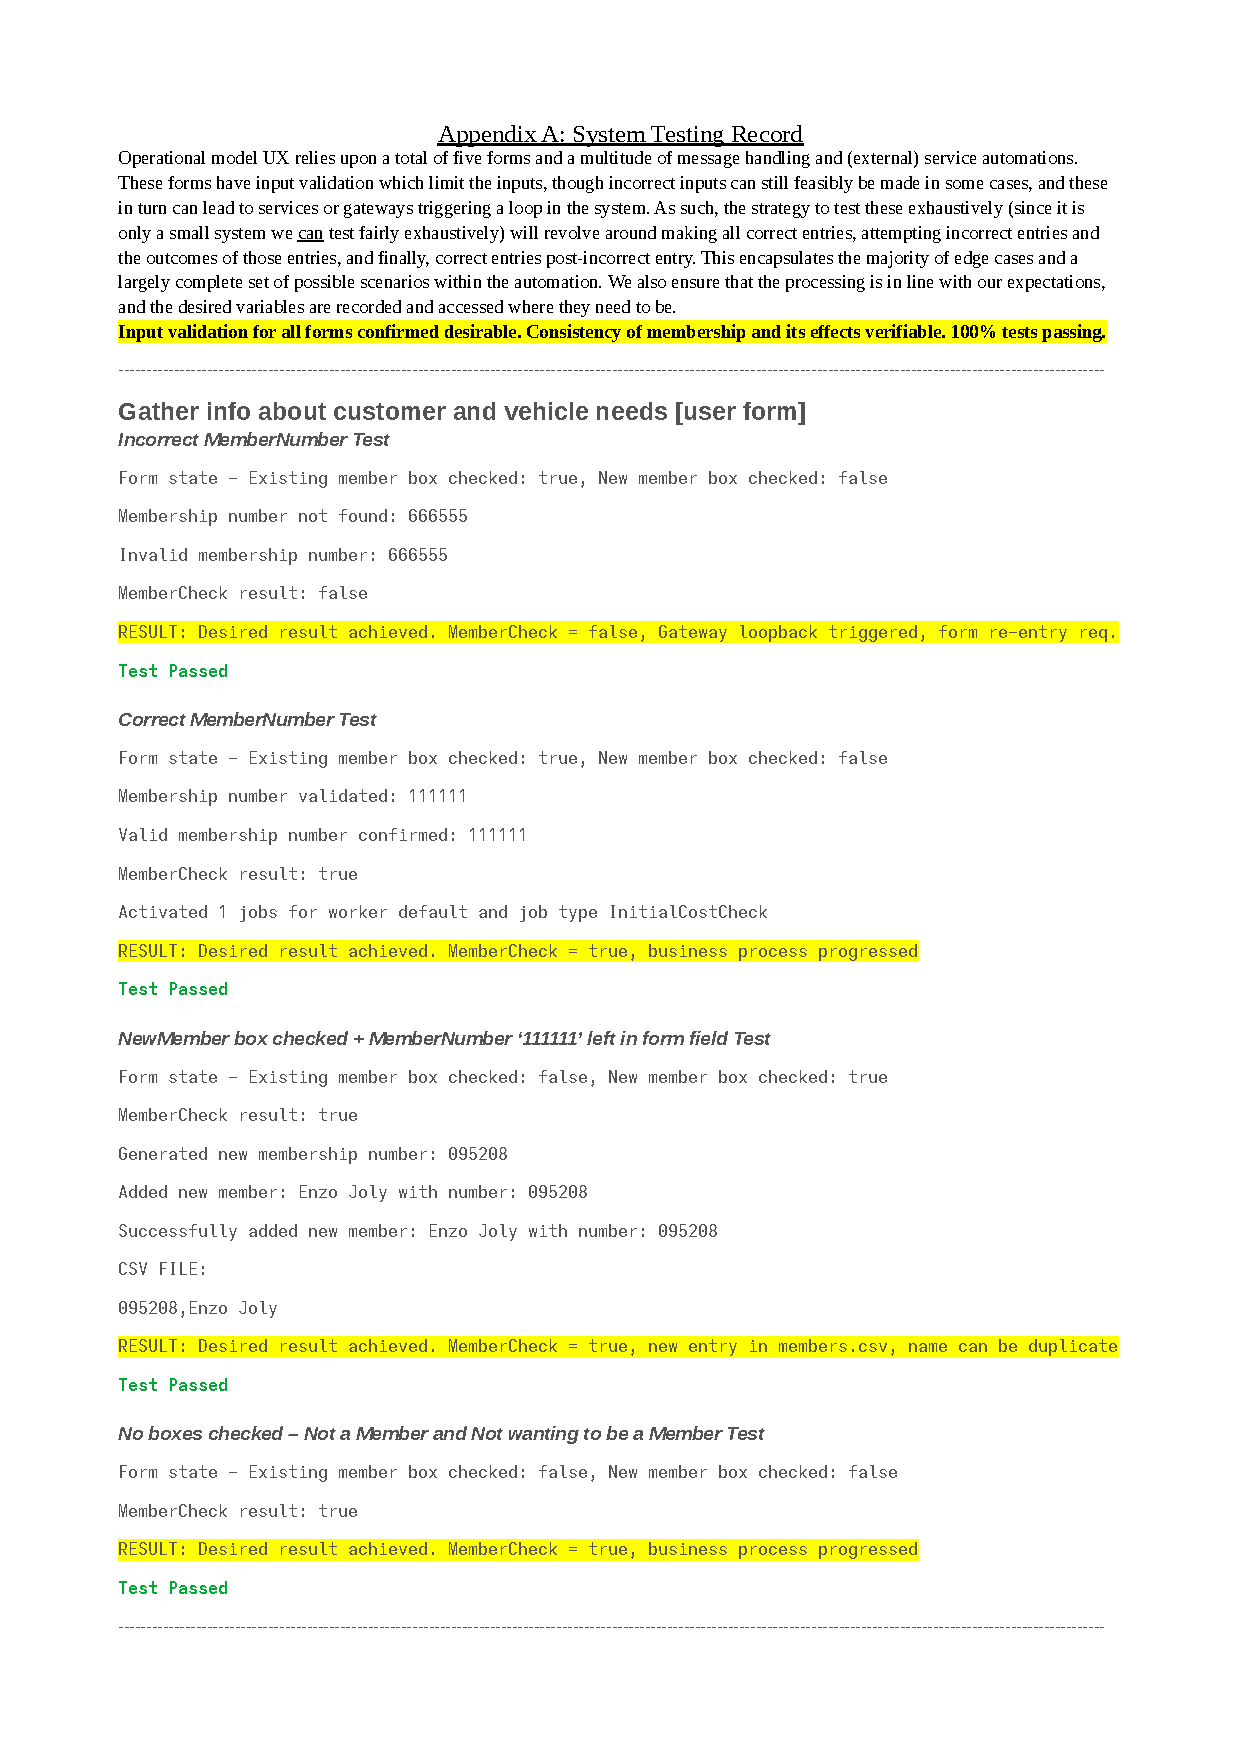
\includepdf[pages=-]{AppendixA.pdf}

\end{document}
